\documentclass{article}

% Document extensibility %
%
% Disables native paragraph indentation
\usepackage{parskip} 
%
% Provides further bullet options for lists
\usepackage{enumitem}

% Mathematical symbol and statement packages %
%
% Necessary
\usepackage{amsmath}
\usepackage{amssymb}
%
% Extensive fraction notation
\usepackage{xfrac}
%
% Generic mathematical commands
% Notable: \degree, \celcius
\usepackage{gensymb}
%
% Variable vector notation (arrow above variable)
\usepackage{esvect}
%
% Multiline boxed equations
\usepackage{empheq}

% Graphic packages %
%
% Diagrams and illustrations
\usepackage{tikz}
\usetikzlibrary{positioning, calc}
%
% Image insertion
\usepackage{graphicx}

% Document content %
%
% Change title of table of contents
\renewcommand{\contentsname}{Units and Vectors}

\title{Homework 1}
\author{Corey Mostero}
\date{Student ID: 256652}

\begin{document}

% Command `\hr` to insert horizontal rules
\newcommand{\hr}{\par\noindent\rule{\textwidth}{0.4pt}}

\maketitle
\newpage

\tableofcontents

\section{Book}

\subsection{1.21}

\begin{tikzpicture}
    \draw[very thick, ->] (0, 0) -- (0, 10) node [above] { $+\hat{y}$ };
    \draw[very thick, ->] (0, 0) -- (10 ,0) node [right] { $+\hat{x}$ };
    \fill (0, 0) circle [radius=2pt] node [above right] { ($0$km,$0$km) };

    \draw[thick, ->, blue] (0, 0) node [left] { Start - $A$ } -- (0, 2.6) node [midway, above, sloped] { $2.6$km } -- (0, 2.6) node [above] { $B$ };
    \draw[thick, ->, blue] (0, 2.6) -- ++(0:4) node [midway, above] { $4.0$km };
    \draw[thick, blue, fill=blue] (4.0, 2.6) -- ++(0:0) node [above] {$C$} -- ++(45:3.1) node [midway, above, sloped] { $3.1$km } -- ++(0:0) circle [radius=2pt] node [above] { End - $D$ };
    \draw[dashed, black] (4.0, 2.6) -- ++(0:2) node [above, midway] { $\theta = 45\degree$ };
\end{tikzpicture}

Variables:
\begin{align*}
    \vv{AB} & = \left((0)\hat{x} + (2.6)\hat{y}\right)\text{km} \\
    \vv{BC} & = \left((4.0)\hat{x} + (0)\hat{y}\right)\text{km} \\
    \|\vv{CD}\| & = 3.1\text{km} \\
    \theta & = 45\degree \\
    \vv{CD}_x & = ? \\
    \vv{CD}_y & = ? \\
    \vv{AD} & = ?
\end{align*}
Finding components of $ \vv{CD} $:
\begin{align*}
    \cos(\theta) & = \frac{\vv{CD}_x}{\text{hyp.}} \\
    \vv{CD}_x & = \text{hyp.} \cdot \cos(\theta) \\
              & = 3.1\text{km} \cdot \cos(45\degree) \\
              & = 2.2\text{km} \\
    \sin(\theta) & = \frac{\vv{CD}_y}{\text{hyp.}} \\
    \vv{CD}_y & = \text{hyp.} \cdot \sin(\theta) \\
              & = 3.1\text{km} \cdot \sin(45\degree) \\
              & = 2.2\text{km}
\end{align*}
$$ \vv{CD} = \left((2.2)\hat{i} + (2.2)\hat{j}\right)\text{km} $$
Finding the vector $ \vv{AD} $:
\begin{align*}
    \vv{AD} & = \vv{AB} + \vv{BC} + \vv{CD} \\
            & = \left(\vv{AB}_x + \vv{BC}_x + \vv{CD}_x\right)\hat{i} + \left(\vv{AB}_y + \vv{BC}_y + \vv{CD}_y\right)\hat{j} \\
            & = \left(0\hat{i} + 4.0\hat{i} + 2.2\hat{i}\right)\text{km} + \left(2.6\hat{j} + 0\hat{j} + 2.2\hat{j}\right)\text{km} \\
            & = \left(6.6\hat{i} + 4.8\hat{j}\right)\text{km}
\end{align*}
Finding magnitude of $ \vv{AD} $:
\begin{align*}
    \|\vv{AD}\| & = \sqrt{(AD_x)^2 + (AD_y)^2} \\
                & = \sqrt{(6.6\text{km})^2 + (4.8\text{km})^2} \\
                & = 8.16\text{km}
\end{align*}
Finding direction of $ \vv{AD} $:
\begin{align*}
    \tan(\theta) & = \frac{\text{opp.}}{\text{adj.}} \\
    \theta & = \arctan\left(\frac{\text{opp.}}{\text{adj.}}\right) \\
           & = \arctan\left(\frac{4.8\text{km}}{2.2\text{km}}\right) \\
           & = 65.38\degree \text{ N of E}
\end{align*}
Solution:
\begin{empheq}[box=\fbox]{align*}
    & \text{Magnitude: } 8.16 \text{km} \\
    & \text{Direction: } 65.38\degree \text{ N of E}
\end{empheq}

\section{Lab Manual}

\subsection{172}

\begin{enumerate}[label=\alph*)]
    \item Prove that $ \vv{A} \cdot \vv{B} = \vv{B} \cdot \vv{A} $
    \item Show that $ \vv{A} \cdot \vv{B} $ can be interpreted either as $ B $ times the component of $ \vv{A} $ in the direction of $ \vv{B} $, or as $ A $ times the component of $ \vv{B} $ in the direction of $ \vv{A} $.
    \item Calculate the dot product of the two vectors, $ \vv{A} \cdot \vv{B} $, given below: (No units)
        \begin{enumerate}[label=\arabic*)]
            \item $ \vv{A} = 20 $ along the +X axis, $ \vv{B} = 15 $ at $ 37\degree $ above the +X axis.
            \item $ \vv{A} = 6 $ at $ 20\degree $ above the +X axis, $ \vv{B} = 10 $ at $ 70\degree $ above the +X axis.
            \item $ \vv{A} = 3 $ along the +X axis, $ \vv{B} = 4 $ along the +X axis.
            \item $ \vv{A} = 4 $ along the +X axis, $ \vv{B} = 4 $ along the -X axis.
            \item $ \vv{A} = 0.3 $ along the +X axis, $ \vv{B} = 0.5 $ at $ 135\degree $ to $ \vv{A} $
            \item $ \vv{A} = 12 $ along the +X axis, $ \vv{B} = 7 $ along the +Y axis.
        \end{enumerate}
\end{enumerate}

a)
\begin{align*}
    \vv{A} \cdot \vv{B} & = \vv{B} \cdot \vv{A} \\
    \vv{A}_x\vv{B}_x + \vv{A}_y\vv{B}_y & = \vv{B}_x\vv{A}_x + \vv{B}_y\vv{A}_y
\end{align*}
Which can be rewritten as
\begin{equation*}
    \boxed{
        \vv{A}_x\vv{B}_x + \vv{A}_y\vv{B}_y = \vv{A}_x\vv{B}_x + \vv{A}_y\vv{B}_y
    }
\end{equation*}

b) \\
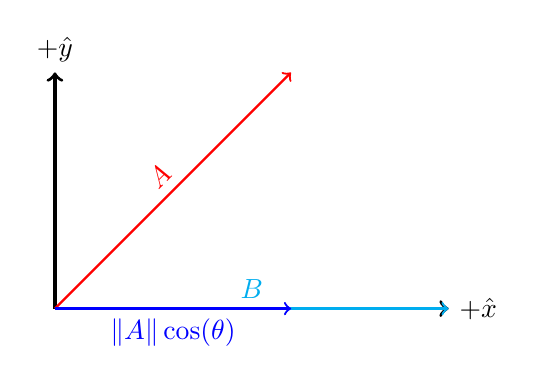
\begin{tikzpicture}
    \draw[very thick, black, ->] (0, 0) -- (0, 3) node [above] { $+\hat{y}$ };
    \draw[very thick, black, ->] (0, 0) -- (5, 0) node [right] { $+\hat{x}$ };
    
    \draw[thick, red, ->] (0, 0) -- ++(45:4.24) node [midway, above, sloped] (A) { $\vv{A}$ };
    \draw[thick, cyan, ->] (0, 0) -- ++(0:5) node [midway, above] (B) { $\vv{B}$ };
    \draw[thick, blue, ->] (0, 0) -- ++(0:3) node [midway, below] (Acos) { $\|\vv{A}\|\cos(\theta)$ };
\end{tikzpicture} \\
The graph illustrates that the projection of $ \vv{A} $ onto $ \vv{B} $ is $ \vv{A}_x $ or otherwise written $ \|\vv{A}\|\cos(\theta) $

Beginning with the dot product
$$ \vv{A} \cdot \vv{B} $$
The projection of $ \vv{A} $ onto $ \vv{B} $ can be seen from above, which can be substituted
\begin{equation*}
    \boxed{
        \|\vv{A}\|\cos(\theta) \cdot \|\vv{B}\|
    }
\end{equation*}
It can now be shown that the dot product can be rewritten as the projection of $ \vv{B} $ times $ \vv{A}_x $ (the component of $ \vv{A} $).

To prove the opposite
$$ \vv{B} \cdot \vv{A} $$
\begin{equation*}
    \boxed{
        \|\vv{B}\|\cos(\theta) \cdot \|\vv{A}\|
    }
\end{equation*}

c)
\begin{enumerate}[label=\arabic*)]
    \item
        \begin{align*}
            \vv{A} & = 20\hat{i} + 0\hat{j} \\
            \|\vv{B}\| & = 15 \text{ at $ 37\degree $ above $ +\hat{x} $ axis} \\
            \vv{A} \cdot \vv{B} & = \|\vv{B}\|\cos(\theta) \cdot \vv{A} \\
                                & = (15)\cos(37)(\sqrt{(20)^2+(0)^2}) \\
                                & = (15)\cos(37)(20) \\
                                & = 239.591
        \end{align*}
        \begin{equation*}
            \boxed{239.6}
        \end{equation*}
    \item
        \begin{align*}
            \|\vv{A}\| & = 6 \text{ at $ 20\degree $ above $ +\hat{x} $ axis} \\
            \|\vv{B}\| & = 10 \text{ at $ 70\degree $ above $ +\hat{x} $ axis} \\
            \theta & = |\theta_{\vv{A}} - \theta_{\vv{B}}| \\
                   & = |20 - 70| \\
                   & = |-50| \\
                   & = 50\degree \\
            \vv{A} \cdot \vv{B} & = \|\vv{B}\|\cos(\theta)\|\vv{A}\| \\
                                & = (10)\cos(50)(6) \\
                                & = 38.567
        \end{align*}
        \begin{equation*}
            \boxed{38.6}
        \end{equation*}
    \item
        \begin{align*}
            \vv{A} & = 3\hat{i} + 0\hat{j} \\
            \vv{B} & = 4\hat{i} + 0\hat{j} \\
            \theta & = 0\degree \\
            \vv{A} \cdot \vv{B} & = \sqrt{(3)^2 + (0)^2}\cos(0)\sqrt{(4)^2 + (0)^2} \\
                                & = (3)(1)(4) \\
                                & = 12.0
        \end{align*}
        \begin{equation*}
            \boxed{12.0}
        \end{equation*}
    \item
        \begin{align*}
            \vv{A} & = 4\hat{i} + 0\hat{j} \\
            \vv{B} & = -4\hat{i} + 0\hat{j} \\
            \theta & = 0\degree \\
            \vv{A} \cdot \vv{B} & = \sqrt{(4)^2 + (0)^2}\cos(0)\sqrt{(-4)^2 + (0)^2} \\
                                & = (4)(1)(4) \\
                                & = 16.0
        \end{align*}
        \begin{equation*}
            \boxed{16.0}
        \end{equation*}
    \item
        \begin{align*}
            \vv{A} & = 0.3\hat{i} + 0\hat{j} \\
            \|\vv{B}\| & = 0.5 \text{ at $ 135\degree $ to $ \vv{A} $} \\
            \theta & = 135\degree \\
            \vv{A} \cdot \vv{B} & = \sqrt{(0.3)^2 + (0)^2}\cos(135)(0.5) \\
                                & = (0.3)\cos(135)(0.5) \\
                                & = -0.106
        \end{align*}
        \begin{equation*}
            \boxed{-0.106}
        \end{equation*}
    \item
        \begin{align*}
            \vv{A} & = 12\hat{i} + 0\hat{j} \\
            \vv{B} & = 0\hat{i} + 7\hat{j} \\
            \theta & = 90\degree \\
            \vv{A} \cdot \vv{B} & = \sqrt{(12)^2 + (0)^2}\cos(90)\sqrt{(0)^2 + (7)^2} \text{, where $\cos(90) = 0$} \\
                                & = 0
        \end{align*}
        \begin{equation*}
            \boxed{0}
        \end{equation*}
\end{enumerate}

\subsection{173 (b)}

Determine the magnitude of $ \vec{A} \times \vec{B} $ in each of the following, and specify the direction as either into or out of the page.

\begin{enumerate}[label=\arabic*)]
    \item
        \begin{align*}
            \|\vv{A}\| & = 10 \\
            \|\vv{B}\| & = 7 \\
            \theta & = 37\degree \\
            \|\vv{A} \times \vv{B}\| & = \|\vv{A}\|\|\vv{B}\|\sin(\theta) \\
                                     & = (10)(7)\sin(37) \\
                                     & = 42.127
        \end{align*}
        \begin{equation*}
            \boxed{42.1 \text{, out}}
        \end{equation*}
    \item
        \begin{align*}
            \|\vv{A}\| & = 20 \\
            \theta_A & = 45\degree \text{ south of $ -\hat{x} $ axis} \\
            \|\vv{B}\| & = 25 \\
            \theta_B & = 0\degree \\
            \theta & = ? \\
            \theta_A & = 45\degree \text{ south of $ -\hat{x} $ axis} = 225\degree \\
            \theta & = |\theta_A - \theta_B| \\
                   & = |270 - 360| \\
                   & = |135|\degree \\
            \|\vv{A} \times \vv{B}\| & = \|\vv{A}\|\|\vv{B}\|\sin(\theta) \\
                                     & = (20)(25)\sin(135) \\
                                     & = 353.553
        \end{align*}
        \begin{equation*}
            \boxed{353.6 \text{, out}}
        \end{equation*}
    \item
        \begin{align*}
            \|\vv{A}\| & = 1 \\
            \|\vv{B}\| & = 3 \\
            \theta & = 90\degree \\
            \|\vv{A} \times \vv{B}\| & = \|\vv{A}\|\|\vv{B}\|\sin(\theta) \\
                                     & = (1)(3)\sin(90) \\
                                     & = 3
        \end{align*}
        \begin{equation*}
            \boxed{3 \text{, in}}
        \end{equation*}
    \item
        \begin{align*}
            \|\vv{A}\| & = 21 \\
            \|\vv{B}\| & = 14 \\
            \theta & = 0\degree \\
            \|\vv{A} \times \vv{B}\| & = \|\vv{A}\|\|\vv{B}\|\sin(\theta) \\
                                     & = (21)(14)\sin(0) \\
                                     & = 0
        \end{align*}
        \begin{equation*}
            \boxed{0 \text{, direction N/A}}
        \end{equation*}
\end{enumerate}

\subsection{174}

Given two vectors, $ \vv{A} = 3\hat{i} + 4\hat{j} - 5\hat{k} $ and $ \vv{B} = -1\hat{i} + 2\hat{j} + 6\hat{k} $
\begin{enumerate}[label=\alph*)]
    \item Find the magnitude of each vector.
    \item Find the angle of each vector to the $ +\hat{x} $ axis.
    \item Find $ \vec{A} \cdot \vec{B} $.
    \item Find the included angle between $ \vec{A} $ and $ \vec{B} $.
    \item Find $ \vec{A} - \vec{B} $. (Leave in component form.)
    \item Find $ \vec{A} \times \vec{B} $. (Leave in component form.)
\end{enumerate}

\begin{enumerate}[label=\alph*)]
    \item
        \begin{align*}
            \|\vec{A}\| & = \sqrt{(A_x)^2 + (A_y)^2 + (A_z)^2} \\
                      & = \sqrt{(3)^2 + (4)^2 + (-5)^2} \\
                      & = 7.071 \\
            \|\vec{B}\| & = \sqrt{(B_x)^2 + (B_y)^2 + (B_z)^2} \\
                      & = \sqrt{(-1)^2 + (2)^2 + (6)^2} \\
                      & = 6.403
        \end{align*}
        \begin{equation*}
            \boxed{
                \|\vec{A}\| = 7.07 \text{, } \|\vv{B}\| = 6.40
            }
        \end{equation*}
    \item
        \begin{align*}
            \cos(\theta_{\vv{A}}) & = \frac{\vv{A}_x}{\sqrt{(\vv{A}_x)^2 + (\vv{A}_y)^2 + (\vv{A}_z)^2}} \\
            \theta_{\vv{A}} & = \arccos\left(\frac{\vv{A}_x}{\sqrt{(\vv{A}_x)^2 + (\vv{A}_y)^2 + (\vv{A}_z)^2}}\right) \\
                   & = \arccos\left(\frac{3}{\sqrt{(3)^2 + (4)^2 + (-5)^2}}\right) \\
                   & = 64.856\degree \\
            \cos(\theta_{\vv{B}}) & = \frac{\vv{B}_x}{\sqrt{(\vv{B}_x)^2 + (\vv{B}_y)^2 + (\vv{B}_z)^2}} \\
            \theta_{\vv{B}} & = \arccos\left(\frac{\vv{B}_x}{\sqrt{(\vv{B}_x)^2 + (\vv{B}_y)^2 + (\vv{B}_z)^2}}\right) \\
                            & = \arccos\left(\frac{-1}{\sqrt{(-1)^2 + (2)^2 + (6)^2}}\right) \\
                            & = 98.985\degree
        \end{align*}
        \begin{equation*}
            \boxed{
                \theta_{\vv{A}} = 64.9\degree \text{, } \theta_{\vv{B}} = 99.0\degree
            }
        \end{equation*}
    \item
        \begin{align*}
            \vv{A} \cdot \vv{B} & = (\vv{A}_x\vv{B}_x) + (\vv{A}_y\vv{B}_y) + (\vv{A}_z\vv{B}_z) \\
                                & = ((3)(-1)) + ((4)(2)) + ((-5)(6)) \\
                                & = -25
        \end{align*}
        \begin{equation*}
            \boxed{-25}
        \end{equation*}
    \item
        \begin{align*}
            \vv{A} \cdot \vv{B} & = -25 \\
            \|\vv{A}\| & = 7.07 \\
            \|\vv{B}\| & = 6.40 \\
            \vec{A} \cdot \vec{B} & = \|\vec{A}\|\|\vec{B}\|\cos(\theta) \\
            \cos(\theta) & = \frac{\vec{A} \cdot \vec{B}}{\|\vec{A}\|\|\vec{B}\|} \\
            \theta & = \arccos\left(\frac{\vec{A} \cdot \vec{B}}{\|\vec{A}\|\|\vec{B}\|}\right) \\
                   & = \arccos\left(\frac{-25}{(7.07)(6.40)}\right) \\
                   & = 123.539\degree
        \end{align*}
        \begin{equation*}
            \boxed{123.5\degree}
        \end{equation*}
    \item
        \begin{align*}
            \vec{A} - \vec{B} & = (\vec{A}_x - \vec{B}_x)\hat{i} + (\vec{A}_y - \vec{B}_y)\hat{j} + (\vec{A}_z - \vec{B}_z)\hat{k} \\
                              & = (3 - (-1))\hat{i} + (4 - 2)\hat{j} + (-5 - 6)\hat{k} \\
                              & = 4\hat{i} + 2\hat{j} - 11\hat{k}
        \end{align*}
        \begin{equation*}
            \boxed{4\hat{i} + 2\hat{j} - 11\hat{k}}
        \end{equation*}
    \item
        \begin{align*}
            \vec{A} \times \vec{B} & =
                \begin{bmatrix}
                    \hat{i} & \hat{j} & \hat{k} \\
                    3 & 4 & -5 \\
                    -1 & 2 & 6
                \end{bmatrix} \\
            & = ((4)(6) - (2)(-5))\hat{i} + ((-1)(-5) - (3)(6))\hat{j} + ((3)(2) - (-1)(4))\hat{k} \\
            & = (34)\hat{i} - (13)\hat{j} + (10)\hat{k}
        \end{align*}
        \begin{equation*}
            \boxed{
                (34)\hat{i} - (13)\hat{j} + (10)\hat{k}
            }
        \end{equation*}
\end{enumerate}

\subsection{184}

In figure 1, 0 is the center of the earth and also the origin, and $ A $ and $ B $ are two points on the earth's surface. As you probably know, the minimum path length (= geodesic) between $ A $ and $ B $ is the circular segment $ D $ of a ``great circle" (= a circle in the plane passing through $ A $, $ B $, and $ O $). Calculating the length, D, of the geodesic is a common navigational problem in sea and air travel, and the scalar (= dot) product provides a simple way to do this without knowing spherical trigonometry. We can find $ D $ from  $ r $ (= radius of the earth) and angle $ a $ (in radians), and we can find $ a $ from the radius vector $ r_A $ of point $ A $ and the radius vector $ r_B $ of point $ B $. (Radius vector means the radius OA or OB written as \textbf{i, j, k} vector.)

\begin{enumerate}[label=(\alph*)]
    \item First, prove that $ \cos(a) $ is given by the expression $ \frac{\left(r_A \cdot r_B\right)}{r^2} $.
    \item In figure 2, the Cartesian coordinates of any point $ P $ on the surface of the sphere are $ (x, y, z) $ and the spherical polar coordinates are $ (r, \theta, \phi) $. Prove from the diagram that
        $$ x = r\sin(\theta)\cos(\phi) $$
        $$ r = r\sin(\theta)\sin(\phi) $$
        $$ z = r\cos(\theta) $$
    \item In figure 2, the latitude (call it gamma, $ \gamma $) of point $ P $ is obviously $ 90 - \theta $ ($ \theta - 90 $ in the northern hemisphere), and the longitude of point $ P $ is $ \phi $ (if we take $ NM $ as the meridian of zero longitude through Greenwich and measure longitude toward the east). Therefore, if we know the latitude and longitude of any point on the surface, we can find its radius vector, $ \vv{r} $. Do this, and so prove that $ \vv{r} $ (to any $ P $) = $ \hat{i}(r\cos(\gamma)\cos(\phi)) + \hat{j}(r\cos(\gamma)\sin(\phi)) + \hat{k}(r\sin(\gamma)) $
    \item New York is at latitude and longitude $ 40.8\degree $ N, $ 74.0\degree $ W (= $ 286.0\degree $ E), and El Camino College is at $ 34.0\degree $ N, $ 118.3\degree $ W. The earth's radius is $ 3960 $ miles (= r). \\
        Prove that:
        $$ \vv{r}_{\text{NY}} = r[\hat{i}(0.209) + \hat{j}(-0.827) + \hat{k}(0.653)] $$
        $$ \vv{r}_{\text{ECC}} = r[\hat{i}(-0.393) + \hat{j}(-0.730) + \hat{k}(0.559)] \text{, and then find angle $ a $} $$
    From this, show that the geodesic distance (ECC to NY) is $ 2450 $ miles ($ 3 $ sig. fig.).
\end{enumerate}

\begin{enumerate}[label=(\alph*)]
    \item Start by expanding the dot product
        $$ \vv{r}_A \cdot \vv{r}_B = \|\vv{r}_A\|\|\vv{r}_B\|\cos(a) $$
        As points $ A $ and $ B $ are both points on earth's surface, their radius will be equal
        $$ \therefore \vv{r}_A = \vv{r}_B = \vv{r} $$
        \begin{align*}
            \cos(a) & = \frac{\|\vv{r}_A\|\|\vv{r}_B\|\cos(a)}{r^2} \\
            r^2\cos(a) & = \|\vv{r}_A\|\|\vv{r}_B\|\cos(a) \\
            \frac{r^2\cos(a)}{\|\vv{r}_A\|\|\vv{r}_B\|} & = \cos(a) \text{, which can be rewritten as} \\
            \frac{\|\vv{r}_A\|\|\vv{r}_B\|\cos(a)}{r^2} & = \cos(a) \\
            \frac{\vv{r}_A \cdot \vv{r}_B}{r^2} & = \cos(a) \\
        \end{align*}
        \begin{equation*}
            \boxed{
                \cos(a) = \frac{\vv{r}_A \cdot \vv{r}_B}{r^2}
            }
        \end{equation*}
    \item
        When first finding $ x $, figure two illustrates that $ x $ is made up from the $ \cos $ of the alternate interior angle $ \phi $ as well as the projection of $ r $ onto the $ \hat{x}/\hat{y} $ axis. This can be written as
        \begin{align*}
            \cos(\phi) & = \frac{x}{r\sin(\theta)} \\
            x & = r\sin(\theta)\cos(\phi)
        \end{align*}
        Similarly when finding $ y $, figure two shows that it is m ade up from the $ \sin $ of the alternate interior angle $ \phi $ of $ y $ over $ r\sin(\theta) $. This can be written as
        \begin{align*}
            \sin(\phi) & = \frac{y}{r\sin(\theta)} \\
            y & = r\sin(\theta)\sin(\phi)
        \end{align*}
        Finally when finding $ z $, figure two shows that $ z $ is simply the projection of $ r $ onto the $ \hat{z} $ axis separated by $ \theta $. This can be written as
        \begin{align*}
            \cos(\theta) & = \frac{z}{r} \\
            z & = r\cos(\theta)
        \end{align*}
    \item
        \begin{align*}
            \gamma & = 90\degree - \theta \\
            \theta & = 90\degree - \gamma \\
            \vec{r} & = \hat{i}x + \hat{j}y + \hat{k}z \\
                    & = \hat{i}(r\sin(\theta)\cos(\phi)) + \hat{j}(r\sin(\theta)\sin(\phi)) + \hat{k}(r\cos(\theta)) \\
                    & = \hat{i}(r\sin(90 - \gamma)\cos(\phi)) + \hat{j}(r\sin(90 - \gamma)\sin(\phi)) + \hat{k}(r\cos(90 - \gamma)) \\
                    & \text{Using the geometric identity that the complementary angle for $ \sin(90 - x) $ is $ \cos(x) $} \\
                    & = \hat{i}(r\cos(\gamma)\cos(\phi)) + \hat{j}(r\cos(\gamma)\sin(\phi)) + \hat{k}(r\sin(\gamma)) \\
        \end{align*}
    \item
        \begin{align*}
            \gamma_{\text{NY}} & = 40.8\degree \\
            \phi_{\text{NY}} & = 286.0\degree \\
            \gamma_{\text{ECC}} & = 34.0\degree \\
            \phi_{\text{ECC}} & = -118.3\degree \\
            r_{\text{earth}} & = 3960 \text{ miles} \\
            \phi_{\text{ECC}} & = -118.3\degree \\
                              & = 360 + (-118.3) \\
                              & = 241.7\degree \\
            \gamma & := \gamma_{\text{NY}} \text{, } \phi := \phi_{\text{NY}} \\
            r_{\text{NY}} & = \hat{i}(r\cos(\gamma)\cos(\phi)) + \hat{j}(r\cos(\gamma)\sin(\phi)) + \hat{k}(r\sin(\gamma)) \\
            r_{\text{NY}} & = r[\hat{i}(\cos(\gamma)\cos(\phi)) + \hat{j}(\cos(\gamma)\sin(\phi)) + \hat{k}(\sin(\gamma))] \\
                          & = r[\hat{i}(\cos(40.8)\cos(286.0)) + \hat{j}(\cos(40.8)\sin(286.0)) + \hat{k}(\sin(40.8))] \\
                          & = r[\hat{i}(0.209) + \hat{j}(-0.827) + \hat{k}(0.653)] \\
            \gamma & := \gamma_{\text{ECC}} \text{, } \phi := \phi_{\text{ECC}} \\
            r_{\text{ECC}} & = \hat{i}(r\cos(\gamma)\cos(\phi)) + \hat{j}(r\cos(\gamma)\sin(\phi)) + \hat{k}(r\sin(\gamma)) \\
            r_{\text{ECC}} & = r[\hat{i}(\cos(\gamma)\cos(\phi)) + \hat{j}(\cos(\gamma)\sin(\phi)) + \hat{k}(\sin(\gamma))] \\
                           & = r[\hat{i}(\cos(34.0)\cos(241.7)) + \hat{j}(\cos(34.0)\sin(241.7)) + \hat{k}(\sin(34.0))] \\
                           & = r[\hat{i}(-0.393) + \hat{j}(-0.730) + \hat{k}(0.559)]
        \end{align*}
        \begin{align*}
            \cos(a) & = \frac{\vv{r_\text{NY}} \cdot \vv{r_\text{ECC}}}{r^2} \\
                    & = \arccos\left(\frac{\vv{r_\text{NY}} \cdot \vv{r_\text{ECC}}}{r^2}\right) \\
                    & = \arccos\left(\frac{r^2((0.209)(-0.393) + (-0.728)(-0.730) + (0.653)(0.559))}{r^2}\right) \\
                    & = \arccos\left((0.209)(-0.393) + (-0.728)(-0.730) + (0.653)(0.559)\right) \\
                    & = 35.479\degree \\
                    & = (35.479\degree)\left(\frac{\pi}{180\degree}\right) \\
                    & = 0.619 \text{ rad}
        \end{align*}
        \begin{align*}
            \text{distance} & = r_{\text{earth}}a \\
                            & = (3960 \text{ miles})(0.619 \text{ rad}) \\
                            & = 2451.24
        \end{align*}
        \begin{equation*}
            \boxed{2450 \text{ miles}}
        \end{equation*}
\end{enumerate}

\end{document}
